% Created 2014-04-14 Mon 18:10
\documentclass[runningheads,a4paper]{llncs}
\usepackage[utf8]{inputenc}
\usepackage[T1]{fontenc}
\usepackage{fixltx2e}
\usepackage{graphicx}
\usepackage{longtable}
\usepackage{float}
\usepackage{wrapfig}
\usepackage{rotating}
\usepackage{amsmath}
\usepackage{textcomp}
\usepackage{marvosym}
\usepackage{wasysym}
\usepackage{amssymb}
\usepackage{hyperref}
\tolerance=1000
\usepackage[usenames,dvipsnames]{xcolor}
\usepackage{epstopdf}
\usepackage{listings}

\urldef{\mailsa}\path|{joel.kuiper, m.a.swertz}@rug.nl|
\urldef{\mailsb}\path|iain.marshall@kcl.ac.uk|
\urldef{\mailsc}\path|byron_wallace@brown.edu|
\institute{University of Groningen P.O. Box 30001, 9700 RB Groningen \\ \mailsa \and King's College London, London SE1 3QD, UK \\ \mailsb \and Brown University, Providence, RI 02906, USA \\ \mailsc}

\begin{document}
\setcounter{tocdepth}{3}
\newcommand{\highlight}[1]{\colorbox{yellow}{#1}}

% Autogenerated, do not edit
\newcommand{\revisiondate}{2014-04-24}
<<<<<<< HEAD
\newcommand{\revision}{3f2c73a}
=======
\newcommand{\revision}{d58899a}
>>>>>>> 1b257ee... updates

\author{Kuiper, J\inst{1}. \and Marshall, I.J.\inst{2} \and Wallace, B.C.\inst{3} \and Swertz, M.A.\inst{1}}
\date{\today}
\title{Spá: a web-based viewer for text mining in Evidence Based Medicine}


\maketitle
\begin{abstract}
Unstructured PDF documents remain the main vehicle for dissemination of scientific findings.
Those interested in gathering and assimilating data must therefore manually peruse published articles and extract from these the elements of interest.
Evidence based medicine provides a compelling illustration of this challenge: many person-hours are spent each year extracting summary information from articles that describe clinical trials.
Machine learning provides a potential means of mitigating this burden by automating extraction.
But, for automated approaches to be useful to end-users, we need tools that allow domain experts to interact with, and benefit from, model predictions.
To this end, we present an open-source tool called Spá\footnote{available under GPLv3 at \url{https://github.com/joelkuiper/spa} \cite{kuiper2014}} that accepts as input an article describing a clinical trial and provides as output an automatically visually annotated rendering of this article.
More generally, Spá provides a framework for visualizing predictions, both at the document and sentence level, for full-text PDFs.
\\
\\
\texttt{revision: \revision, date: \revisiondate}
\end{abstract}

\section{Introduction}
\label{section:intro}
Identifying and extracting specific elements of interest from the full-texts of published articles is an important practical step for many tasks.
Consider evidence based medicine (EBM) \cite{sackett1996}, in which the aim is to address a specific clinical question by identifying and synthesizing data from all published relevant articles.
Thus when undertaking such exercises, one needs, e.g., to extract from the article describing a clinical trial the number of participants that were enrolled (the sample size).
Another component of EBM is assessing the \emph{risk of bias} for a particular study across different domains.
For example, one often wants to assess the risk of bias due to improper blinding of participants and personnel.
For this task, one wants both to make a summary judgement (e.g., low risk of bias) while simulteanously extracting the sentences supporting this assessment.

%Finding sentences or words with particular characteristics within a larger document is an important task in natural language processing and machine learning. For example, one may wish to identify the most important sentences in a document to automatically generate a summary, or match a certain ontology to impose a certain structure.

Extracting such information from the free text of articles describing clinical trials is a laborious process.
Machine learning methods provide the machinery to automate such extractions: these can effectively impose the structure of interest onto PDF's.
But if such technologies are to be practically useful, we need tools to visualize the predicted annotations.
Here we describe Spá which aspires to realize this aim.
Spá is an open-source, web-based tool that incorporates state-of-the-art machine learning predictors to automatically annotate PDF articles describing clinical trials with risk-of-bias predictions and extracted sample sizes.
This tool is useful for practitioners of evidence based medicine and other biomedical researchers.

\begin{figure}[htb]
\centering
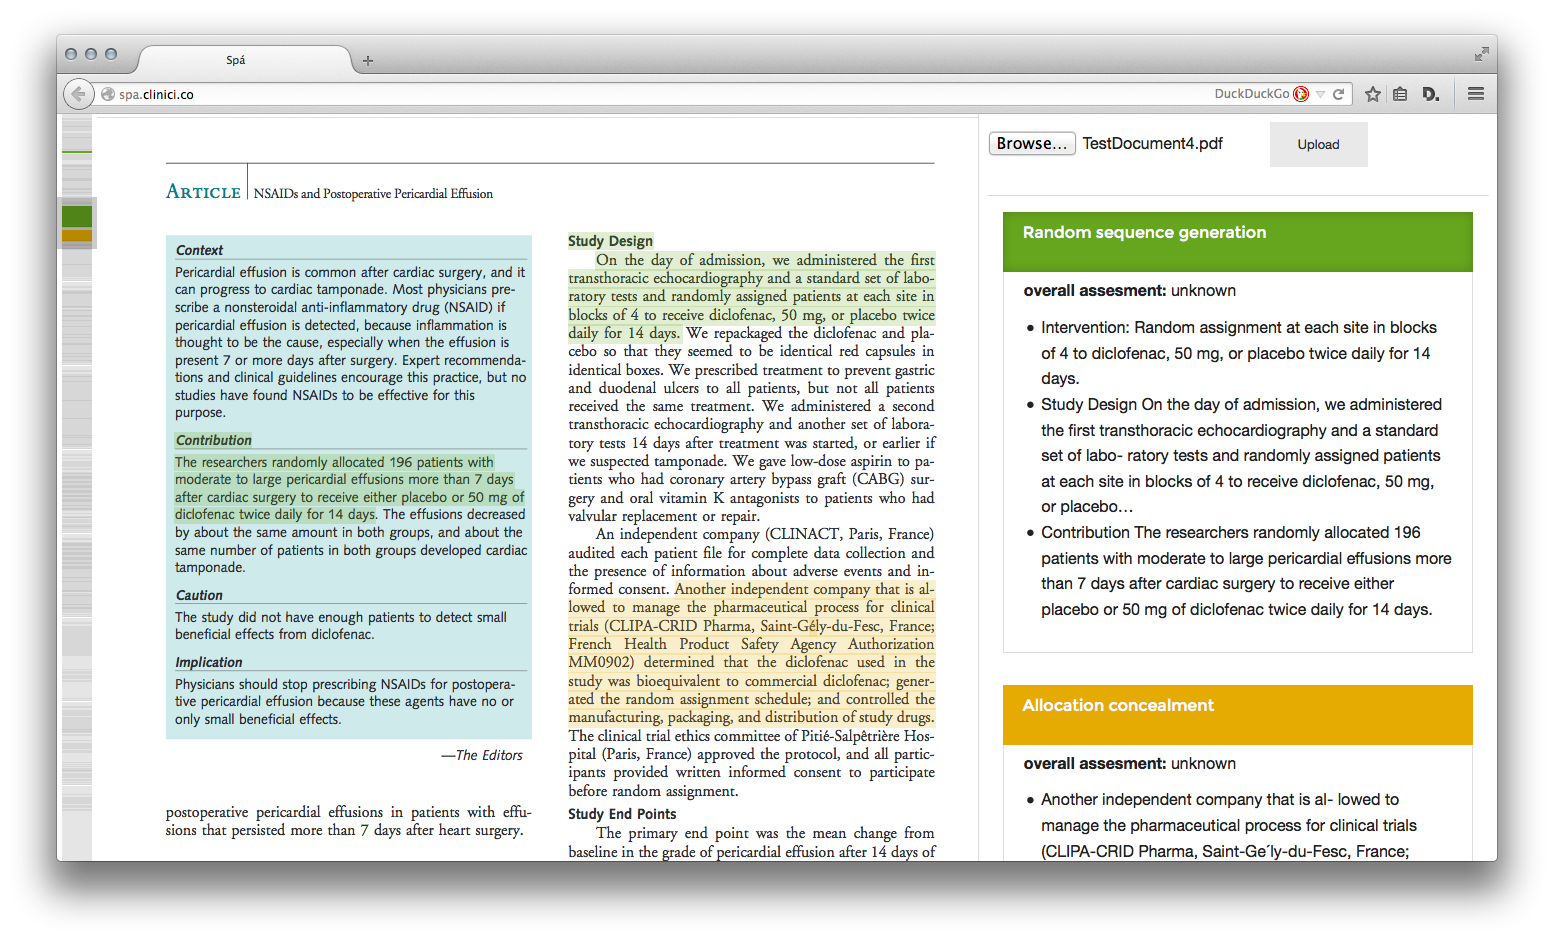
\includegraphics[width=.9\linewidth]{./images/screenshot.png}
\end{figure}

While our application of interest is evidence based medicine, we emphasize that the framework can incorporate other types of articles (and the appropriate trained machine learning models).
Thus the contribution of this work is two-fold, as we present: (1) a practical tool that incorporates cutting edge machine learning to help biomedical researchers rapidly assess published articles describing clinicals, and, (2) a general open-source web framework for visualizing the predictions of trained models from full-text articles.
These contributions are described further in Sections \ref{section:EBM-ML} and \ref{section:architecture}, respectively.

\section{Automating Evidence-Based Medicine}
\label{section:EBM-ML}

\subsection{Systematic Reviews}
The process of pooling and summarizing clinical trials is called \emph{systematic reviewing}, and forms the corner-stone of current evidence based medical practice.
Systematic reviewing consists of specifying an inclusion criteria, searching the literature, screening the retrieved citations to identify eligible studies and, finally, summarizing the relevant evidence.
But achieving this aim is complicated by the massive numbers of trials that are conducted: for example, the Cochrane Library alone indexes 286,418 trials as having been conducted in the last decade \cite{valkenhoef2012}.
While publishing standards are improving and novel tools for systematic reviewing are being created to address this problem \highlight{citation needed}, a lot of legacy publications will remain only as PDF documents.
This raises questions about the sustainability of systematic reviews in its current form.

To aid the process of systematic reviewing we made a generic web-based tool that allows the visualization of annotations within a PDF documents, or meta-information alongside it.
The aim is to have a pluggable system to allow for semi-automated (machine assisted) screening, data extraction and data summarization.

\subsection{Machine Learning Strategies}

\begin{itemize}
\item Basically show that we're using state of the art
\item Briefly talk about cochrane DB / distant supervision
\item KDD stuff (briefly)
\item Multi-task stuff!
\end{itemize}

\section{Architecture overview}
\label{section:architecture}
\begin{figure}[htb]
\centering
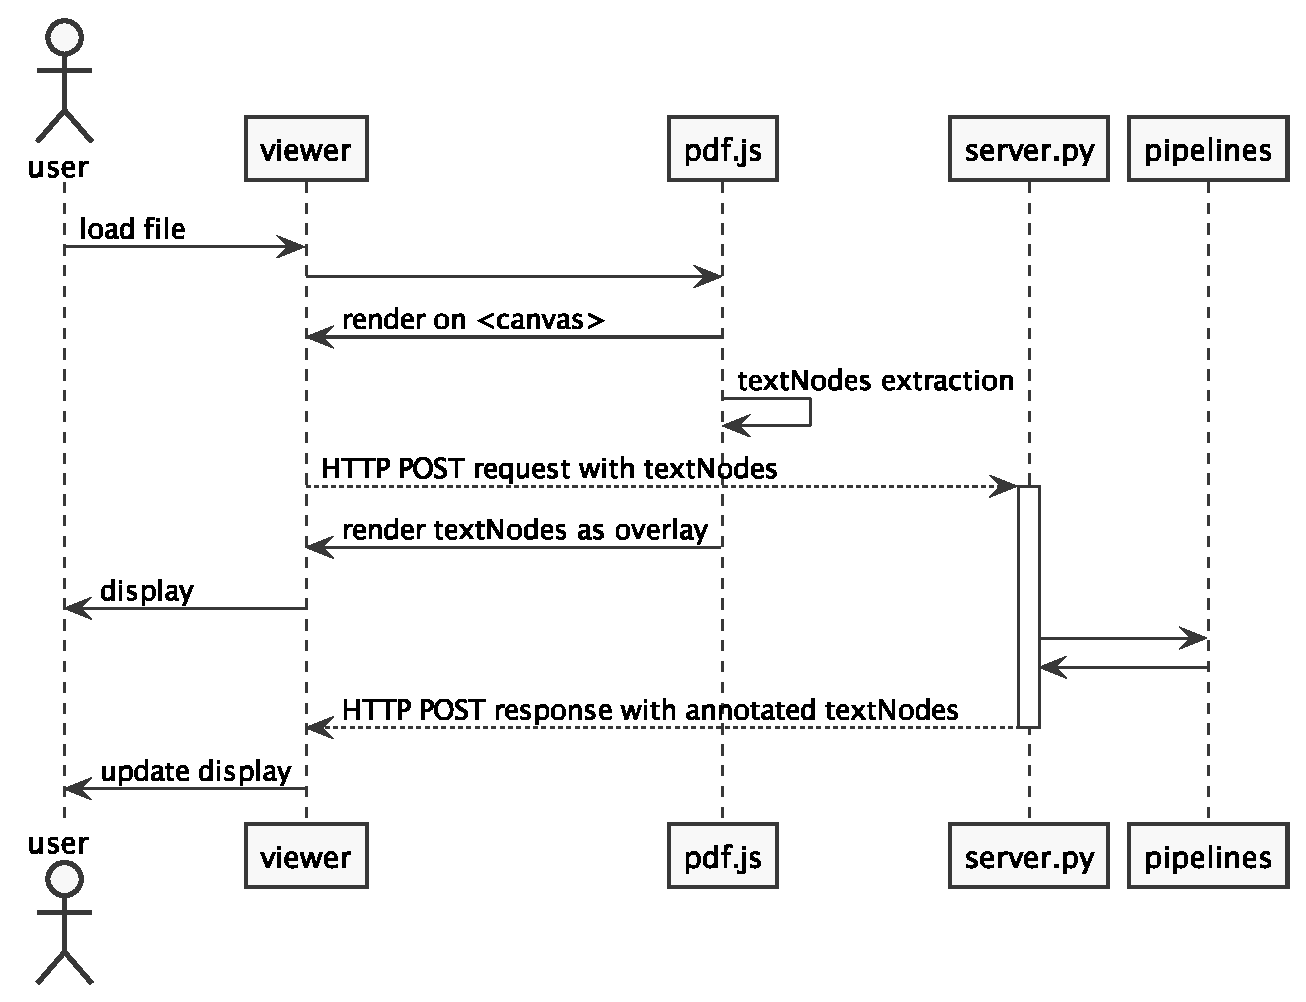
\includegraphics[width=.9\linewidth]{./diagrams//sequence.eps}
\caption{\label{fig:sequence}Sequence diagram of a typical request-response}
\end{figure}
Spá relies on Mozilla pdf.js\footnote{\url{http://mozilla.github.io/pdf.js}} for visualization of the document and text extraction.
The results of the text extraction are processed by the Python server-side by a variety of (pluggable) pipelines, as outlined in figure \ref{fig:sequence}.
Results from these pipelines, which could be complicated machine learning systems, are communicated back to the browser and displayed using React components \footnote{\url{http://facebook.github.io/react/}}.

\section{Conclusion \& Future work}
We present a web-based tool for interactive visualization of annotations and metadata on PDF documents.
This allows users to see the results from machine learning systems within the context of a specific document.
Moreover, we present a case study for Evidence Based Medicine by automatically extracting potential Risks of Bias, with supporting sentences.

However, we believe the tool to be useful for a much wider range of text mining and machine learning applications.
To increase the generality of the tool work is being done to support a consumer/producer protocol for the pipelines, allowing developers to quickly plug in new systems.
Furthermore, work is being done on allowing users to save selected annotations, possibly embedded within the document itself, for sharing and off-line use.

\subsubsection{Acknowledgments}
Part of this research was funded from the European Union Seventh Framework Programme (FP7/2007-2013) under grant agreement n° 261433 (Biobank Standardisation and Harmonisation for Research Excellence in the European Union - BioSHaRE-EU)

\bibliographystyle{splncs}
\bibliography{references}

\end{document}
